% !TEX root = ../main.tex

\chapter{相关工作} \label{ch:related}

如第\ref{sec:compcertbackend}节中所述,在经验证的编译器领域,许多工作是围绕CompCert编译器开展的。
我们将在第\ref{sec:relatedc}节中对CompCert及它的扩展CompCertSSA中端进行介绍。
在本章第\ref{sec:relatedf}节中,我们将对已有的针对函数式语言编译器的形式化验证工作进行介绍。
它们大部分还是基于CompCert完成的。 
国内外的研究者们已经注意到使函数式编译器复用基于SSA中间语言的基础设施后端的重要性。
在第\ref{sec:relatedssa}节中,我们对基于SSA中间语言的LLVM编译框架以及经验证的LLVM IR进行了介绍。
我们的工作基于对这些相关工作的观察建立,是朝着构建利用SSA中间语言优势的经验证的函数式编译器迈出的第一步。

\section{经验证的编译器框架CompCert} \label{sec:relatedc}

经验证的C语言编译器CompCert提供了对编译器正确性进行形式化验证的理论和框架~\cite{leroy2009formally}。
它的大体编译流程如图\ref{fig:compcert}所示。该图是CompCert编译链图的简化版本,
省略了一些编译步骤,主要保留了我们在后文中介绍基于CompCert的工作时需要了解的中间语言和编译步骤。
本文中的工作所使用的基于模拟的验证技术是CompCert框架中提供的。
\begin{figure}[htbp]
    \centering
    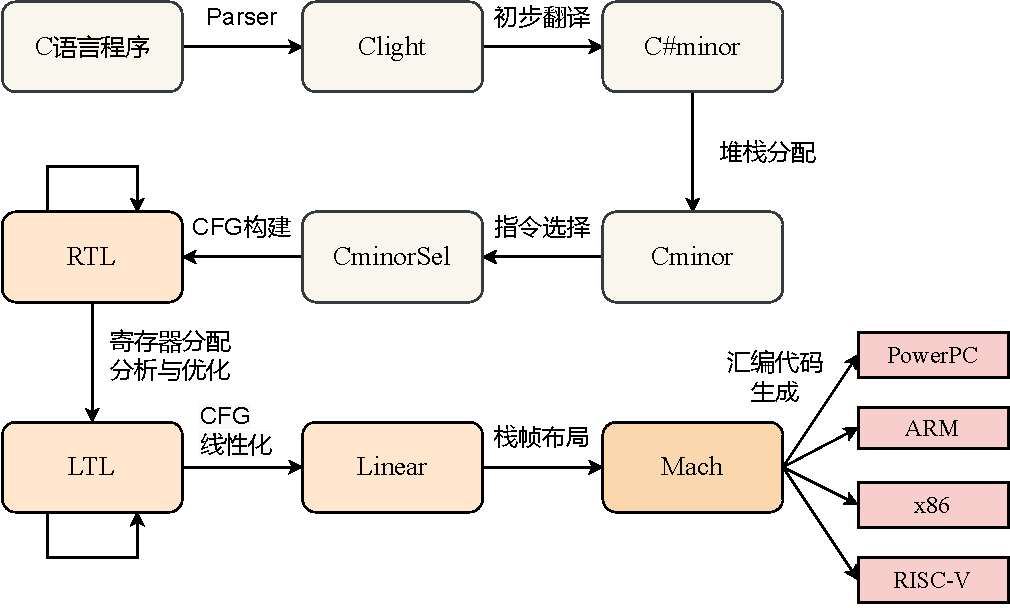
\includegraphics[width=0.8\linewidth]{figures/compcert.pdf}
    \caption{CompCert编译链概览}\label{fig:compcert}
\end{figure}

CompCertSSA是CompCert的一个扩展,具有一个基于SSA的中间端~\cite{compcertssa}。
它将SSA作为一种可选的优化中间语言,允许在RTL(Register Transfer Language)三地址代码和SSA中间语言之间进行转换。
CompCertSSA将RTL语言转换为SSA,经过全局值编号(Global Value Numbering,GVN)优化,再转换回RTL。
GVN优化是指对相同值的变量赋予相同的编号,从而消除冗余的计算。这里的SSA程序状态与RTL程序状态类似,
但是寄存器和当前函数类型要进行修改。在CompCertSSA中,$\phi$函数没有放在基本代码块中,
$\phi$指令代码块与普通指令构成的基本块是平行的结构。它们的语义也是平行定义的,
对基本代码块的控制流图定义了小步操作语义,对$\phi$指令代码块定义了大步操作语义。

虽然这使得CompCert能够实现一些基于SSA的优化~\cite{compcertssa-op,blazy-cpp2023},
但是CompCertSSA提供的优化仍然比较有限,不能与LLVM的后端优化相媲美。
本文中的SSA目标语言选择了接近LLVM中间语言的形式,也是为了对经验证的函数式语言编译器复用LLVM后端优化提供基础。
不过,它提供了一个从C语言开始的经过完整验证的编译链,是开发针对SSA的经验证的函数式编译器的有力工具。


\section{经验证的函数式编译器} \label{sec:relatedf}

许多经验证的函数式编译器选择与CompCert相连接~\cite{belanger2019certified, dargaye2009verification}。
经验证的函数式编译器CertiCoq将Gallina(Coq语言)编译到了CompCert中使用的的Clight~\cite{belanger2019certified}。
miniML经验证的编译器也使用了CompCert框架,将其编译到了CompCert中的中间语言Cminor~\cite{dargaye2009verification}。
也有经验证的函数式编译器选择了独立完成到汇编语言的编译链,例如CakeML~\cite{cakeml2016}。

\begin{itemize}
    \item \textbf{Gallina经验证的编译器CertiCoq:} 
    CertiCoq将Gallina编译到了C语言的子集Clight,以便与CompCert链接起来并最终编译到汇编语言,
    从而获得一个完整的经过验证的编译链~\cite{belanger2019certified,zoe-oopsla2021,zoe-icfp2021}。
    在CertiCoq中,源程序被转换为CPS形式后,经历了反柯里化(Uncurrying)、$\lambda$提升($\lambda$ Lifting)
    等优化~\cite{li2018verifying},并进行了闭包转换(Closure Conversion)~\cite{paraskevopoulou2019closure},
    确保函数没有包含非全局作用域的自由变量。之后,经过前述处理后得到的CPS程序就被转换到了Clight。
    尽管CertiCoq中使用的CPS语言,即L6语言,是一种纯函数式的语言,但是经过了前述的转换过程,
    研究者们能够较为直接地找出它与Clignt的对应关系。
    L6程序中的一个函数就对应着Clight中的一个函数。L6中所有的调用都是尾调用(Tail Call),并且C语言
    编译器CompCert实现了尾调用优化,可以将尾调用转换为跳转,不用创建新的栈帧。
    由于C语言没有自动的垃圾收集器(Garbage Collection),CertiCoq构造了与经验证的收集器的接口,
    并验证了该接口的正确性~\cite{wang2019certifying}。

    从CPS到Clight的编译过程及其形式化证明在Coq中实现,不过其使用的是大步操作语义而不是小步操作语义。
    其转换算法的正确性也使用了基于模拟的方法进行证明,证明了L6到Clight程序的前向模拟性质。
    该编译器的目标语言不是基于SSA的,因此不能直接连接到LLVM框架,也不能利用基于SSA中间语言的优化。
    \item \textbf{miniML经验证的编译器前端MLCompCert:} 
    MLCompCert是Zaynah Dargaye等人设计的一个经验证的编译器前端~\cite{dargaye2009verification}。
    它的源语言是ML纯函数式语言的部分,即miniML,包括了$\lambda$演算、$let$绑定、模式匹配等。
    它的目标语言是CompCert编译器后端的中间语言Cminor,即一种类似于C语言的底层语言。
    该编译器实现了一些经典的函数式程序编译优化,例如反柯里化和统一数据结构表示等。
    设计者们在Coq中对该函数式程序编译器前端进行了实现和验证。
    \item \textbf{经验证的函数式语言编译器CakeML:} 
    该编译器使用的源程序CakeML语言贴近实际中使用的函数式编程语言~\cite{cakeml2016}。
    它支持用户定义的模块、相互递归函数和模式匹配(Pattern Matching)等语言特性。
    CakeML编译器支持高效的柯里化多参数函数、可配置的数据表示、展开调用栈的异常、寄存器分配等功能。
    经过十几种中间语言的编译及优化过程,它最终将函数式语言编译到了机器码,支持32位及64位的ARM、RISC-V等不同架构。
    CakeML编译器为了提升寄存器分配的性能,会在进行寄存器分配之前对程序使用一个类似SSA化的转换,
    减小变量的生存期。由此转换步骤产生的程序并不严格符合SSA形式,它没有$\phi$函数。
    它使用隐式的$\phi$函数消除,用变量的移动替换$\phi$函数。
    该编译器的开发过程在HOL4定理证明工具中完成。
\end{itemize}


\section{基于SSA中间语言的编译器} \label{sec:relatedssa}

基于SSA的中间语言(例如LLVM IR)模块化、可移植和优化潜能大等特性引起了函数式编译器开发者的关注。
近年来,一些原本不使用SSA后端的函数式编译器已经开始转向SSA后端以获得更好的性能~\cite{farvardin2020new}。
在经验证的编译器领域,研究者们为了使用LLVM编译框架的优势,开始为LLVM IR提供形式化语义~\cite{zhao2012formalizing}。

\begin{itemize}
    \item \textbf{LLVM编译器框架:} 
    CertiCoq将Gallina编译到了C语言的子集Cligh
    \item \textbf{SML-New Jersey基于LLVM编译器后端的版本:} 
    SML-New Jersey编译器(SML/NJ)是Standard ML的著名编译器。在最近发布的新版本中,它更改了后端,
    将CPS中间语言编译到了LLVM IR~\cite{farvardin2020new}。CPS程序首先被转换为控制流图(Control-Flow Graph, CFG)中间语言,
    然后再转换为LLVM IR。这是因为将CPS中间语言连接到基于SSA的编译器基础设施能够利用这些编译器提供的丰富后端优化。
    但这项工作不是经过形式化验证的。
    我们的工作受到了这一趋势的启发,并进一步尝试对这种连接进行形式化验证。
    \item \textbf{经验证的LLVM IR: Vellvm:} 
    Vellvm在定理证明工具Coq中定义了LLVM中间语言的抽象语法树(Abstract Syntax Tree, AST),并为LLVM IR提供了形式化语义。
    早期版本的Vellvm提供了LLVM IR的操作语义~\cite{zhao2012formalizing},
    而在较新版本中已迁移到了基于交互树(Interactive Tree, ITree)的语义~\cite{zakowski2021modular}。
    在本文第\ref{sec:overview}节所介绍的编译链中,SSA程序首先被编译到了Vellvm AST,然后生成了最终的LLVM IR程序。
\end{itemize}
